\documentclass[11pt]{scrartcl}

\title{Anforderungsspezifikation}
\author{Silvan Adrian \\ Fabian Binna}
\date{\today{}}

\usepackage[ngerman]{babel}
\usepackage[automark]{scrpage2}
\usepackage[colorlinks = true,
linkcolor = black]{hyperref}
\usepackage{color}
\usepackage[normalem]{ulem}
\usepackage{scrpage2}
\usepackage{graphicx}
\usepackage{tabularx}
\usepackage{longtable, tabu}
\graphicspath{ {../22_Grafiken/01_Logo/}{images/}{../../22_Grafiken/01_Logo/} }
\pagestyle{scrheadings}

\clearscrheadfoot
\ihead{
\includegraphics[scale=0.3]{SDDC}}
\ohead{Projekt: SDDC}
\ifoot{Anforderungsspezifikation}
\cfoot{Version: 1.05}
\ofoot{Datum: \today{}}
\setheadsepline{0.5pt}
\setfootsepline{0.5pt}

\usepackage{ucs}
\usepackage[utf8]{inputenc}
\usepackage[T1]{fontenc}


\begin{document}
\def\arraystretch{1.5}
\begin{titlepage}
\begin{center}
\vspace{10em}

\includegraphics[scale=2]{SDDC}
\vspace{10em}
\end{center}
\begin{center}
\huge {Anforderungsspezifikation}
\end{center}
\begin{center}
\vspace{10em}
\LARGE {Silvan Adrian} \\
\LARGE {Fabian Binna}
\end{center}

\end{titlepage}

\newpage
\section{Änderungshistorie}
\begin{tabularx}{\linewidth}{l l X l}
\textbf{Datum} & \textbf{Version} & \textbf{Änderung}  & \textbf{Autor} \\
\hline
\textbf{02.10.15} & 1.00 & Erstellung des Dokuments & Gruppe \\
\textbf{02.10.15} & 1.01 & Nicht funktionale Anforderungen & Silvan Adrian\\
\textbf{02.10.15} & 1.02 & Use Cases Aktoren + User Stories Aktoren & Silvan 
Adrian\\
\textbf{03.10.15} & 1.03 & Anforderungen API & Fabian Binna\\
\textbf{03.10.15} & 1.04 & Anforderungen Dashboards + Mockups eingefügt & Silvan 
Adrian\\
\textbf{03.10.15} & 1.05 & Use Cases fully dressed & Silvan Adrian\\

\end{tabularx}

\newpage
\tableofcontents
\newpage

\section{Einführung}
\subsection{Zweck}
Dieses Dokument beinhaltet die Anforderung zur Analyse.
\subsection{Gültigkeitsbereich}
Dieses Dokument ist während des ganzen Projekts gültig.


\subsection{Referenzen}
-

\section{Anforderungen}
\subsection{API}
Die API definiert einen Workflow der einen Service auf einer Cloud erstellt. Es ist offen, ob 
dieser Service über mehrere Cloud Anbieter hinaus geht. Der Service wird durch 
ein Konfigurationsfile (z.B. json) definiert. Zusätzlich können Scriptfiles referenziert werden, 
die die Software auf den Instanzen installieren. Ein Service kann auch wieder gelöscht werden.
 Es ist nicht die Aufgabe der API existierende Services zu identifizieren. 
 Die API muss Modular sein, das heisst es sollte möglich sein andere oder eigene 
 Programme für die Cloud Kommunikation zu verwenden. Innerhalb der API 
 werden Compute, Storage, Network usw. als ServiceModule bezeichnet. 
 Diese Abstraktion ermöglicht das wiederverwenden und erweitern der API.
\newpage
\subsection{Customer-Dashboard}
\subsubsection{Homescreen}
Im Homescreen (sobald der Customer auf das Dashboard zugreift) werden alle zu 
Verfügung stehenden Services angezeigt.
Hier werden die Services Offerings genannt um eine Unterscheidung zwischen 
Abonnierten Services (Services) und zur Verfügung stehenden Services (Offerings) 
machen zu können.

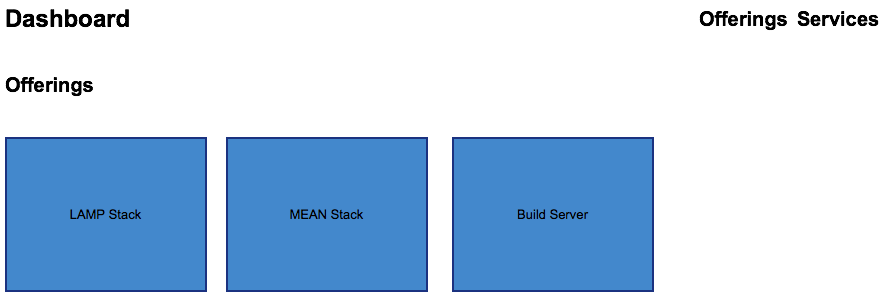
\includegraphics[width=\textwidth]{homescreen_customer}

\subsubsection{Services Übersicht}
In der Services Übersicht werden dem Customer alle abonnierten Services 
angezeigt und können hier auch gekündigt werden.

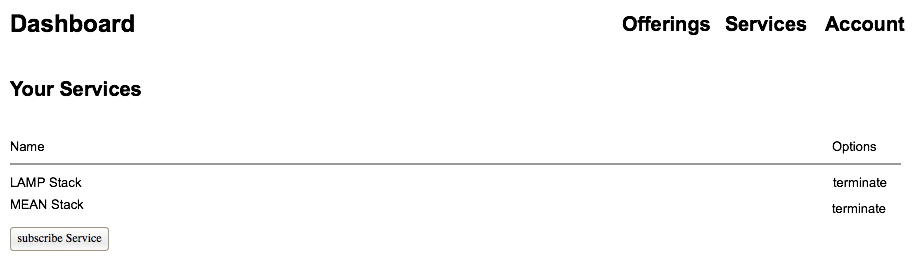
\includegraphics[width=\textwidth]{services_overview}


\subsubsection{Service abonnieren}
Sobald ein Service auf dem Homescreen ausgewählt wird muss noch der zuständige 
Provider gewählt werden (häng auch wieder davon ab von welchem Provider bisher Logindaten hinterlegt 
wurden).
Da momentan noch kein Hybrid Betrieb vorgesehen ist muss ein Account gewählt 
werden unter welchem der Service verrechnet wird.
\begin{figure}[h]
  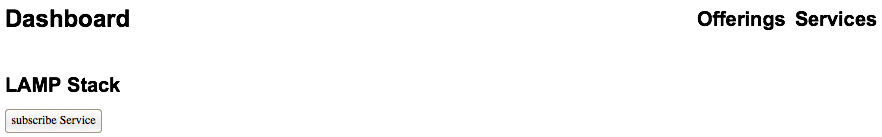
\includegraphics[width=\textwidth]{service_settings}
\end{figure}

\newpage
\subsubsection{Cloud Credentials}
Da für jeden Provider wieder Logindaten benötigt werden müssen diese an einer 
zentralen Stelle gespeichert werden (anhand von denen kann sich auch das Service Angebot 
ändern).
\begin{figure}[h]
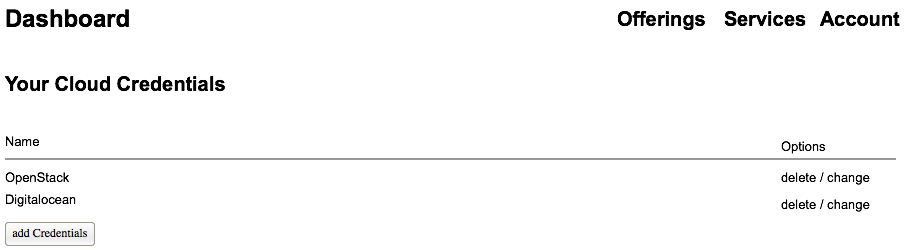
\includegraphics[width=\textwidth]{service_accounts}
\end{figure}
\subsection{Admin-Dashboard}
Zusätzlich zum Customer-Dashboard soll ein Admin-Dashboard zur Verfügung stellen 
in welchem der Admin Services und Servicemodule erstellen kann.

\subsubsection{Service}
Ein Service hat einen bestimmten Namen und jedem Service sind eine gewisse 
Anzahl Servicemodule zugeteilt. um den Service abbilden zu können.
Hier kann der Admin den Service ändern und je nach Anforderung den Service 
anpassen.

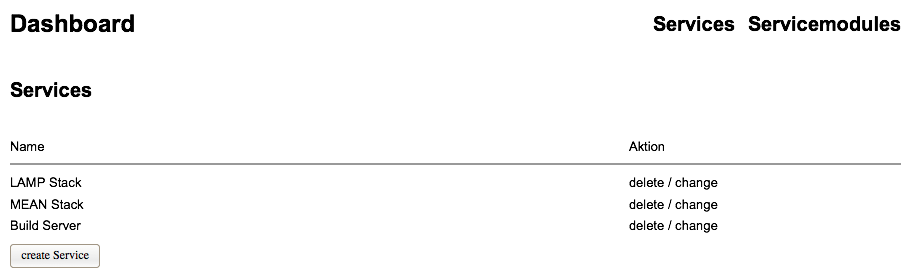
\includegraphics[width=\textwidth]{homescreen_admin}

\subsubsection{Servicemodul}
Jedes Servicemodul besitzt einen Namen und wird einem Provider zugeschrieben, 
dabei kann jedes Servicemodule den Typ Compute,Network oder Storage haben.

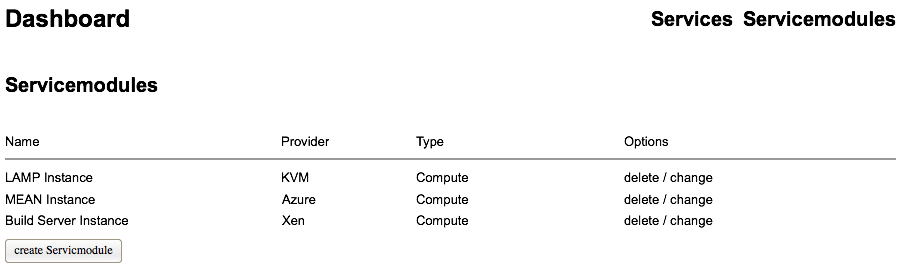
\includegraphics[width=\textwidth]{servicemodules_admin}

\section{Use Cases}
\subsection{Use Case Diagramm}
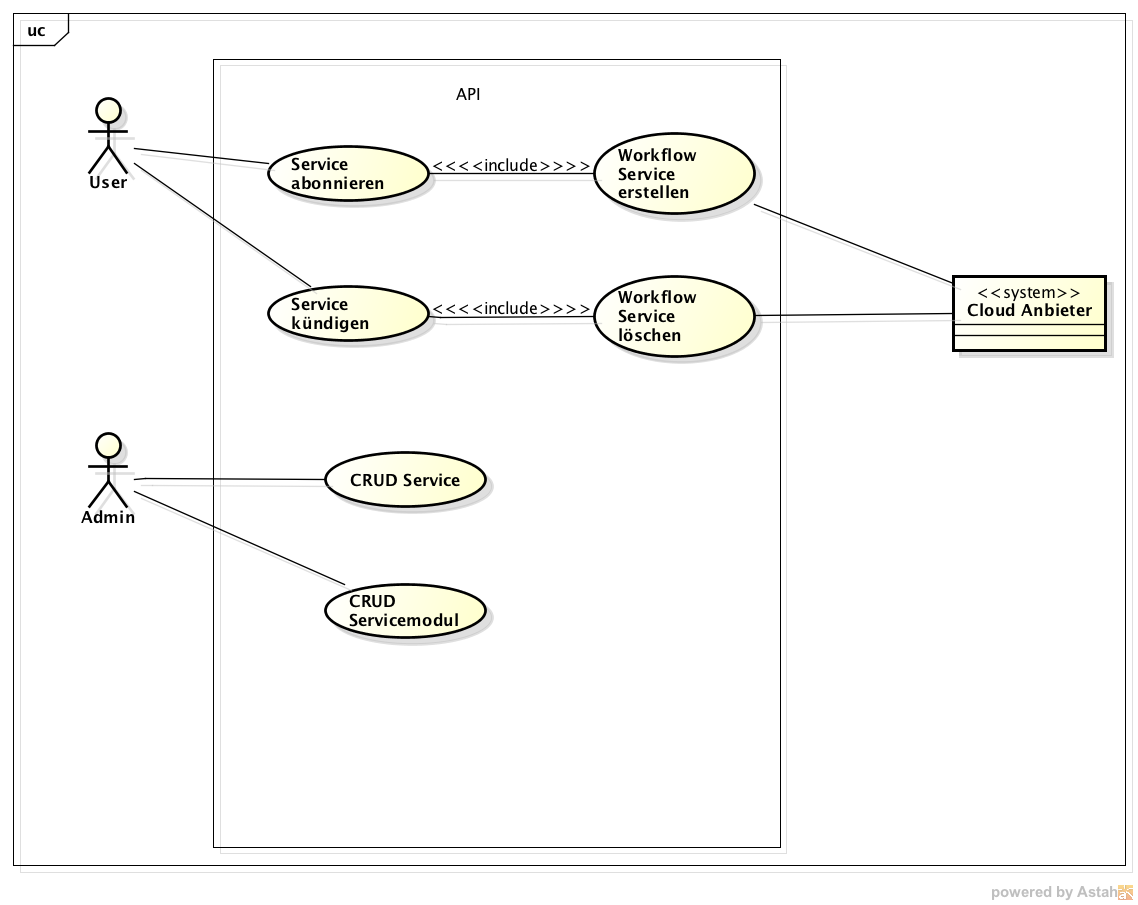
\includegraphics[width=\textwidth]{UseCase-Diagramm}
\subsection{Aktoren \& Stakeholders}
\subsubsection{Customer}
Als Customer möchte ich meine abonnierten Services verwalten.
\\
\begin{tabularx}{\linewidth}{l l X }
  \textbf{Aktor} & \textbf{Typ} & \textbf{Ziele}\\
  \hline
  Customer & Primary & 
  \begin{minipage}{5in}
  \vskip 4pt
  \begin{itemize}
    \item Service abonnieren
    \item Service kündigen
    \item Cloud Logindaten hinzufügen
    \item Cloud Logindaten anpassen
    \item Cloud Logindaten löschen
  \end{itemize}
  \vskip 4pt
 \end{minipage}\\
 \hline
\end{tabularx}


\subsubsection{Admin}
Als Admin möchte ich Services und Servicemodule verwalten können.
\\
\begin{tabularx}{\linewidth}{l l X }
  \textbf{Aktor} & \textbf{Typ} & \textbf{Ziele}\\
  \hline
  Admin & Primary & 
  \begin{minipage}{5in}
  \vskip 4pt
  \begin{itemize}
    \item Service erstellen
    \item Service anpassen
    \item Service löschen
    \item Servicemodul erstellen
    \item Servicemodul anpassen
    \item Servicemodul löschen
  \end{itemize}
  \vskip 4pt
 \end{minipage}\\
 \hline
\end{tabularx}

\newpage
\subsection{Beschreibungen fully dressed}
%Serve abonnieren begin
\subsubsection{UC01: Service abonnieren}
\belowtabulinesep = 1mm
\begin{longtabu} to \textwidth {X[1,l] X[2,l]}
	\bfseries Primäraktor & Customer  \\\hline 
	\bfseries Steakholders und Interessen & Customer: Möchte einen Service abonnieren  \\\hline 
	\bfseries Vorbedingungen & Das Customer-Dashboard wurde geöffnet, ist bei der API authentifiziert und 
	hat einen Cloud Account hinzugefügt. \\\hline 
	\bfseries Nachbedingungen & Die Service Infos wurden gespeichert und der Workflow wurde angestossen  
	\\\hline 
	\bfseries Standartablauf & 
		\begin{enumerate}
			\item Der Customer gibt die Webadresse für das Dashboard ein
			\item Wiederholen bis kein Service mehr abonniert werden soll
			\begin{enumerate}
			    \item Der Customer wechselt in die \textbf{Offerings Übersicht}
			    \item Der Customer wählt einen der vorhanden \textbf{Services} aus
			    \item Der Customer wählt einen vorhanden \textbf{Account} auf welchem er den \textbf{Service}
			abonnieren will
			    \item Der Customer drückt den Button \textbf{subscribe Service}
			    \item Der Customer wird in die \textbf{Services Übersicht} weitergeleitet
			\end{enumerate}
		\item Der Customer schliesst das Customer-Dashboard
		\end{enumerate}
      \\\hline
      	\bfseries Alternativer Ablauf & 
		\begin{enumerate}
		  
		\item
		  \begin{enumerate}
		    \item Der Customer entscheidet sich um und schliesst das 
		    Fenster/Tab
		    
		  \end{enumerate}
		  
		  \item 
                 \begin{enumerate}
		    \item Der Customer entscheidet sich um
		    \begin{enumerate}
		      \item Schliesst das Fenster/Tab
		    \end{enumerate}
		    \item  Der Customer entscheidet sich um
		     \begin{enumerate}
		      \item Schliesst das Fenster/Tab
		      \item geht zurück in die \textbf{Offerings Übersicht}
		    \end{enumerate}
		    
		       \item  Der Customer entscheidet sich um
		     \begin{enumerate}
		      \item Schliesst das Fenster/Tab
		      \item geht zurück in die \textbf{Offerings Übersicht}
		      \item wählt einen anderen Account
		    \end{enumerate}
		    
		    
		     \item  Der Customer entscheidet sich um
		     \begin{enumerate}
		      \item Schliesst das Fenster/Tab
		      \item geht zurück in die \textbf{Offerings Übersicht}
		      \item wählt einen anderen Account
		    \end{enumerate}
		    
		  \end{enumerate}
			
		\end{enumerate}
	 \\\hline
	\bfseries Spezielle Anforderungen & siehe nichtfunktionale Anforderungen  \\\hline 
	\bfseries Technologie- und Datenvarianten & Keine  \\\hline 
	\bfseries Auftrittshäufigkeit & mehrmals pro Woche  \\\hline 
	\bfseries Offene Fragen & Keine  \\\hline  
\end{longtabu}
%Serve abonnieren end
\newpage
%Service kündigen begin
\subsubsection{UC02: Service kündigen}
\begin{longtabu} to \textwidth {X[1,l] X[2,l]}
	\bfseries Primäraktor & Customer  \\\hline 
	\bfseries Steakholders und Interessen & Customer: Möchte einen Service kündigen  \\\hline 
	\bfseries Vorbedingungen & Das Customer-Dashboard wurde geöffnet, ist bei der API authentifiziert und 
	hat einen Service abonniert  \\\hline 
	\bfseries Nachbedingungen & Die Service Infos wurden gelöscht und der Workflow wurde angestossen   \\\hline 
	\bfseries Standartablauf & 
		\begin{enumerate}
			\item Der Customer gibt die Webadresse für das Dashboard ein
			\item Wiederholen bis kein Service mehr gekündigt werden soll
			\begin{enumerate}
			    \item Der Customer wechselt in die \textbf{Services Übersicht}
			    \item Der Customer wählt einen der vorhanden \textbf{Services} aus
			    \item Der Customer drückt auf den link \textbf{terminate}
			    \item Der Customer wird in die \textbf{Services Übersicht} weitergeleitet
			\end{enumerate}
		\item Der Customer schliesst das Customer-Dashboard
		\end{enumerate}
      \\\hline
      	\bfseries Alternativer Ablauf & 
		\begin{enumerate}
		  
		\item
		  \begin{enumerate}
		    \item Der Customer entscheidet sich um und schliesst das 
		    Fenster/Tab
		  \end{enumerate}
		  \item 
                 \begin{enumerate}
		    \item Der Customer entscheidet sich um
		    \begin{enumerate}
		      \item Schliesst das Fenster/Tab
		    \end{enumerate}
		    \item  Der Customer entscheidet sich um
		     \begin{enumerate}
		      \item Schliesst das Fenster/Tab
		      \item wählt einen anderen Service
		    \end{enumerate}
		    
		       \item  Der Customer entscheidet sich um
		     \begin{enumerate}
		      \item Schliesst das Fenster/Tab
		      \item wählt einen anderen Service
		    \end{enumerate}
		    
		  \end{enumerate}
			
		\end{enumerate}
	 \\\hline

      \\\hline
	\bfseries Spezielle Anforderungen & siehe nichtfunktionale Anforderungen  \\\hline 
	\bfseries Technologie- und Datenvarianten & Keine  \\\hline 
	\bfseries Auftrittshäufigkeit & mehrmals pro Woche  \\\hline 
	\bfseries Offene Fragen & Keine  \\\hline  
\end{longtabu}
%Service kündigen end
\newpage
%Cloud Logindaten verwalten begin
\subsubsection{UC03: Cloud Logindaten verwalten}
\begin{longtabu} to \textwidth {X[1,l] X[2,l]}
	\bfseries Primäraktor & Customer  \\\hline 
	\bfseries Steakholders und Interessen & Customer: Möchte ich Cloud Logindaten verwalten  \\\hline 
	\bfseries Vorbedingungen & Das Customer-Dashboard wurde geöffnet  \\\hline 
	\bfseries Nachbedingungen & Die Account Infos wurden gespeichert  \\\hline 
	\bfseries Standartablauf & 
		\begin{enumerate}
			\item Der Customer gibt die Webadresse für das Dashboard ein
			\item Der Customer wechselt in die \textbf{Account/Cloud Credentials Übersicht}
			\item Solange wiederholen bis kein Account mehr hinzugefügt werden muss
			  \begin{enumerate}
			    \item Customer drückt Button \textbf{Add Credentials}
			    \item Customer füllt gefragt Felder aus
			    \item Customer bestätigt Eingaben mit Klick auf \textbf{Save}
			  \end{enumerate}
			\item Der Customer schliesst das Customer-Dashboard
		\end{enumerate}
      \\\hline
      \bfseries Alternativer Ablauf & 
      \begin{enumerate}
          \setcounter{enumi}{2}
            \item 
            \begin{enumerate}
              \item Wiederholen bis kein Account mehr geändert werden muss
                \begin{enumerate}
                  \item Account auswählen und auf \textbf{change} Link klicken
                  \item Felder anpassen
                  \item Änderungen bestätigen mit Klick auf Button \textbf{Save}
                \end{enumerate}
                \item Wiederholen bis kein Account mehr gelöscht werden muss
                \begin{enumerate}
                  \item Account auswählen und auf \textbf{delete} Link klicken
                \end{enumerate}
            \end{enumerate}
            
      \end{enumerate}
      
      \\\hline
	\bfseries Spezielle Anforderungen & siehe nichtfunktionale Anforderungen  \\\hline 
	\bfseries Technologie- und Datenvarianten & Keine  \\\hline 
	\bfseries Auftrittshäufigkeit & mehrmals pro Woche  \\\hline 
	\bfseries Offene Fragen & Keine  \\\hline  
\end{longtabu}
%Cloud Logindaten verwalten end
%Services verwalten begin
\subsubsection{UC04: Services verwalten}

\begin{longtabu} to \textwidth {X[1,l] X[2,l]}
	\bfseries Primäraktor & Customer  \\\hline 
	\bfseries Steakholders und Interessen & Admin: Möchte einen Service verwalten  \\\hline 
	\bfseries Vorbedingungen & Das Admin-Dashboard wurde geöffnet und Admin eingeloggt, 
	falls Service gelöscht werden soll darf kein Customer mehr den Service abonniert haben\\\hline 
	\bfseries Nachbedingungen & Das Admin-Dashboard wurde geschlossen und Änderungen 
	wurden gespeichert  \\\hline 
	\bfseries Standartablauf & 
		\begin{enumerate}
			\item Der Admin gibt die Webadresse für das Admin-Dashboard ein
			\item Wiederholen bis kein neuer Service hinzugefügt werden muss
			\begin{enumerate}
			  \item Der Admin wechselt in die \textbf{Services Übersicht}
			  \item Der Admin drückt auf den button \textbf{create Service}
			  \item Der Admin füllt die benötigten Daten ein \textbf{(Name, welche Servicemodule)}
			  \item der Admin bestätigt mit Klick auf Button \textbf{Save}
			\end{enumerate}
		\end{enumerate}
      \\\hline
      \bfseries Alternativer Ablauf & 
      \begin{enumerate}
        \setcounter{enumi}{1}
        \item 
        \begin{enumerate}
          \item Wiederholen bis kein Service mehr geändert werden muss
            \begin{enumerate}
              \item Service auswählen und auf Link \textbf{change} klicken
              \item Daten ändern
              \item Durch Klick auf Button \textbf{Save} bestätigen
            \end{enumerate}
            \item Wiederholen bis kein Service mehr gelöscht werden muss
            \begin{enumerate}
              \item Service auswählen und Link \textbf{löschen} auswählen
            \end{enumerate}
        \end{enumerate}
      \end{enumerate}
      \\\hline
	\bfseries Spezielle Anforderungen & siehe nichtfunktionale Anforderungen  \\\hline 
	\bfseries Technologie- und Datenvarianten & Keine  \\\hline 
	\bfseries Auftrittshäufigkeit & mehrmals pro Woche  \\\hline 
	\bfseries Offene Fragen & Keine  \\\hline  
\end{longtabu}
%Services verwalten end
\newpage
%Servicemodule verwalten begin
\subsubsection{UC05: Servicemodule verwalten}
\begin{longtabu} to \textwidth {X[1,l] X[2,l]}
	\bfseries Primäraktor & Customer  \\\hline 
	\bfseries Steakholders und Interessen & Admin: Möchte ein Servicemodul verwalten  \\\hline 
	\bfseries Vorbedingungen & Das Admin-Dashboard wurde geöffnet und Admin eingeloggt, 
	falls Servicemodul gelöscht werden soll darf kein Service mehr das Servicemodul verwenden. \\\hline 
	\bfseries Nachbedingungen & Das Admin-Dashboard wurde geschlossen und 
	Änderungen wurden gespeichert \\\hline 
	\bfseries Standartablauf & 
	\begin{enumerate}
			\item Der Admin gibt die Webadresse für das Admin-Dashboard ein
			\item Wiederholen bis kein neues Servicemodul hinzugefügt werden muss
			\begin{enumerate}
			  \item Der Admin wechselt in die \textbf{Servicemodules Übersicht}
			  \item Der Admin drückt auf den button \textbf{create Servicemodule}
			  \item Der Admin füllt die benötigten Daten ein \textbf{(Name, Provider,Typ)}
			  \item der Admin bestätigt mit Klick auf Button \textbf{Save}
			\end{enumerate}
		\end{enumerate}
      \\\hline
      \bfseries Alternativer Ablauf & 
      \begin{enumerate}
        \setcounter{enumi}{1}
        \item 
        \begin{enumerate}
          \item Wiederholen bis kein Servicemodul mehr geändert werden muss
            \begin{enumerate}
              \item Servicemodul auswählen und auf Link \textbf{change} klicken
              \item Daten ändern
              \item Durch Klick auf Button \textbf{Save} bestätigen
            \end{enumerate}
            \item Wiederholen bis kein Servicemodul mehr gelöscht werden muss
            \begin{enumerate}
              \item Service auswählen und Link \textbf{löschen} auswählen
            \end{enumerate}
        \end{enumerate}
      \end{enumerate}
      \\\hline

	\bfseries Spezielle Anforderungen & siehe nichtfunktionale Anforderungen  \\\hline 
	\bfseries Technologie- und Datenvarianten & Keine  \\\hline 
	\bfseries Auftrittshäufigkeit & mehrmals pro Woche  \\\hline 
	\bfseries Offene Fragen & Keine  \\\hline  
\end{longtabu}
%Servicemodule verwalten end
\newpage
\section{User Stories}
\subsection{Rollen}
\subsubsection{User}
Als User benutze ich das Dashboard, um mir einen Service zu abonnieren und 
\subsubsection{Admin}
Als Admin benutze ich die API über die Kommandozeile oder nutze das 
Admin-Dashboard um neue Services zusammenzustellen.



\section{Nichtfunktionale Anforderungen}
\subsection{Menge}
\begin{itemize}
  \item Die Software unterstützt mehr als 30 Cloud Anbieter (libcloud)
  \item Bei jedem Cloud Anbieter bestehen eine gewisse Anzahl Services (von Anbieter zu Anbieter verschieden)
\end{itemize}

\subsection{Schnittstellen}
\begin{itemize}
  \item Die Software wird über HTTP/HTTPS angesprochen
  \item Zur Interaktion im Admin-Dashboard werden die herkömmlichen 
  Schnittstellen gebraucht (Maus,Tastatur,Bildschirm)
  \item Interaktionen können auch über die Kommandozeile ausgeführt werden
\end{itemize}
\subsection{Qualitätsmerkmale}
\subsubsection{Funktionalität}
siehe Abschnitt API und Dashboard
\subsubsection{Zuverlässigkeit}
\begin{itemize}
  \item Der Workflow zum erstellen eines Services soll entweder durchgeführt und 
  abgeschlossen werden oder falls Unterbruch/Fehler rückgängig gemacht 
  werden.
  \item Die Software soll verteilt betrieben werden und eine möglichst hohe 
  Verfügbarkeit bieten
\end{itemize}
\subsubsection{Benutzerbarkeit}
\begin{itemize}
  \item Die Software kann über das vorgesehene Admin-Dashboard benutzt werden
  \item Die API kann auch über die Kommandozeile angesprochen werden
\end{itemize}
\subsubsection{Effizienz}
\begin{itemize}
  \item 
\end{itemize}
\subsubsection{Änderbarkeit}
Die Software soll modular aufgebaut werden, damit Erweiterungen in Zukunft 
problemlos möglich sind.
\subsubsection{Übertragbarkeit}
Das Projekt wird in Python geschrieben ist somit also auf Python mindestens in der Version 2.5 angewiesen, 
kann allerdings durch den Einsatz eines Docker Containers einfach Übertragbar 
gemacht werden.
\end{document}